\section{Experimental setup}
\begin{figure}[H]
        \centering
        \def\svgwidth{\textwidth}
       \input{../img/aufbau.pdf_tex}
        \caption{Experimental setup for the measurement of energy and decay time of cosmic muons.
        Muons are detected in a tank (filled with a scintillating fluid), causing flashes of light while flying through.
        The amount of light emitted is determined with photomultipliers,
        their signal then sent to a system of evaluating
        devices and recorded by multi channel analyzers.}
        \label{img:setup}
\end{figure}
\autoref{img:setup} shows the setup that was used in the experiment.
Its main part is a big metal tank filled with 470\,l of a liquid scintillator.
The flashes of light which are caused by the muons when they travel through the scintillator
are measured with two photomultipliers located at the edges of the cylindrical tank (PMl and PMr).
The signal from the two photomultipliers is then amplified with two \emph{linear amplifiers}.
The gain of the amplifiers is set to 2.
From these amplifiers, the signal goes into \emph{discriminators}.
They only let pass signals with an amplitude exceeding an adjustable threshold.
This threshold is set to a value which lets pass about 1000 pulses per second for each scintillator,
in order to cut off underground noise but also to let through enough desired muon signals.
The output signal of the discriminators is a rectangular pulse of about 50\,ns length and -1.0\,V amplitude.
\autoref{img:pmladisc} shows a pulse from PMr (yellow), the amplified signal (blue)
and the output of the discriminator (pink).
\begin{figure}[H]
\begin{center}
  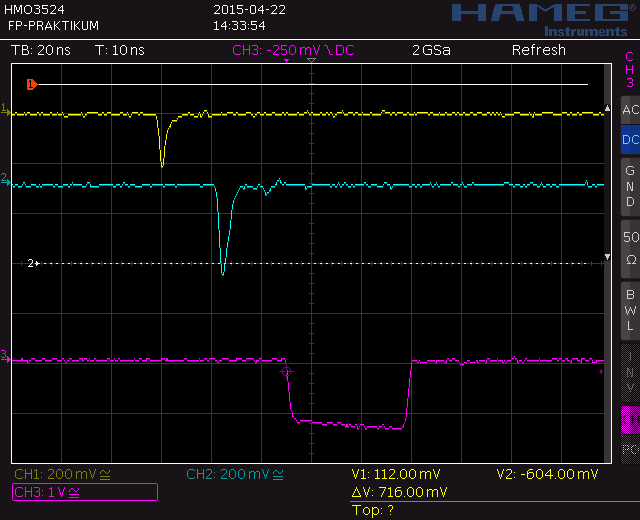
\includegraphics[width=0.5\textwidth]{../img/S0011.PNG}
  \caption{A muon passing through the scintillator causes a pulse of the photomultiplier PMr (yellow),
  the signal is then amplified (blue) and passes the discriminator
  which provides a rectangular output signal (pink).}
  \label{img:pmladisc}
\end{center}
\end{figure} 
The signals of the two discriminators are collected in a \emph{coincidence unit} (AND I).
The output signal of the coincidence unit is also a digital pulse like the one of the discriminators
and it is triggered only if two signals from the discriminators reach its inputs simultaneously.
This configuration again blocks a lot of undesired underground signals,
since it is assumed that a muon passing the tank will generate a signal in both photomultipliers at once.
A counter (Z I) after the coincidence unit permits the determination of the number of coinciding signals
over a specific period.
\autoref{img:discdiscandI} shows a sample of those signals
(the signal from the discriminators in yellow and blue and the output of the coincidence unit in pink).
\begin{figure}[H]
\begin{center}
  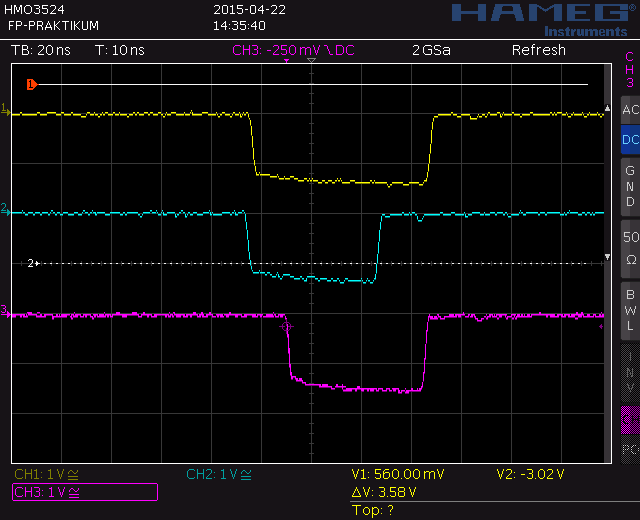
\includegraphics[width=0.5\textwidth]{../img/S0012.PNG}
  \caption{Coinciding signals from the discriminators (yellow and blue) create a pulse
  of the coincidence unit AND I (pink).}
  \label{img:discdiscandI}
\end{center}
\end{figure}
In order to determine the energy of the muon, the analog signals of the linear amplifiers
also take a second way in the circuit:
The signals are \emph{added} and then delayed by 170\,ns in a \emph{delay generator}
(to await analysis of the signals in a different part of the setup, this will become clear later).
\autoref{img:lalaadddel} shows the described signals, from the amplifiers in yellow and blue,
the sum signal in pink and the delayed signal in green.
\begin{figure}[H]
\begin{center}
  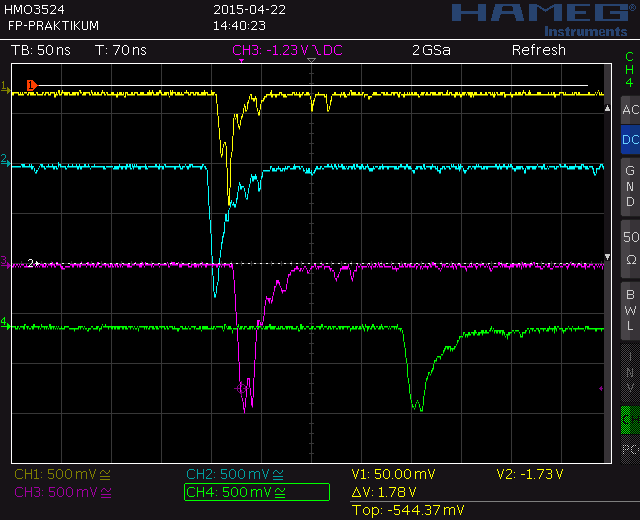
\includegraphics[width=0.5\textwidth]{../img/S0013.PNG}
  \caption{A muon causes peaks after the amplifiers (yellow and blue). The peaks are added (pink)
  and delayed (green).}
  \label{img:lalaadddel}
\end{center}
\end{figure}
After the delay generator, the signal goes over a \emph{capacitor} (to block the constant component of the signal)
and into a \emph{linear gate}.
The control signal for the gate comes from a different part of the setup and it is being triggered
if the approach a muon has been detected over and in the scintillating tank.
\autoref{img:delcapgate} shows a signal before the capacitor (yellow), after it (blue),
the control signal for the linear gate (pink) and the output signal of the gate (green).
On the figure it can be seen clearly that a signal can only pass the gate if it is open:
The first peak of the blue signal can not pass, but the second runs through the gate,
since it is opened by the pink pulse.
The additional two small peaks of the green signal occur due to the opening and closing of the gate
and constitute the main cause of the \emph{pedestal} which is measured in the course of the experiment.
\emph{Pedestal} refers to the nonzero amplitude coming from the linear gate after opening
even if there is no incoming signal.
\begin{figure}[H]
\begin{center}
  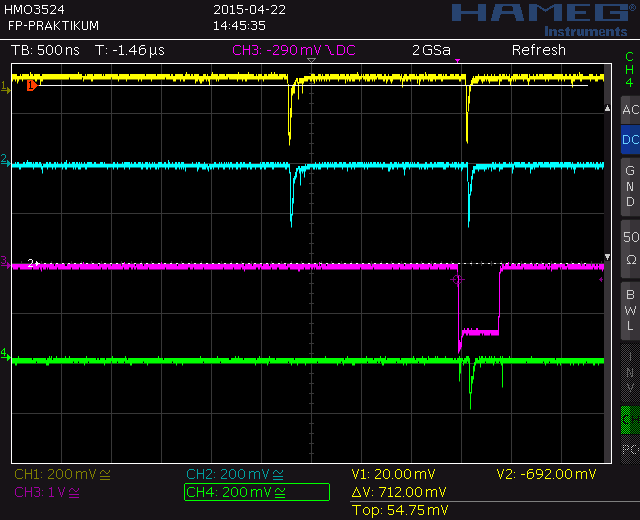
\includegraphics[width=0.5\textwidth]{../img/S0014.PNG}
  \caption{Signature of muon decay in the tank: The first peak is caused by the incoming muon,
  the second by the electron originating in the decay of the muon after 1.8\,\textmu s.
  The signals are measured before the capacitor (yellow) and after the capacitor (blue).
  The control signal for the linear gate is depicted in pink and the output of the linear gate in green.
  The first signal can not pass the gate because the control signal is not supplied.}
  \label{img:delcapgate}
\end{center}
\end{figure}
An \emph{attenuator} after the linear gate damps the signal.
The attenuation for the main measurement is -12\,dB in order not to overload the following \emph{shaping amplifier}
which shows nonlinear behaviour above an input signal of about 100\,mV.

\autoref{img:gateattshamp} shows the signal from the linear gate (yellow), the attenuated signal (blue) and
the signal from the shaping amplifier (pink).
The shaping amplifier integrates and differentiates its input signal and yields an output signal
whose maximum amplitude is proportional to the charge of the input signal.

After the shaping amplifier a \emph{multi channel analyzer} ranks the pulses by their amplitude
and sends the data to a computer.

\begin{figure}[H]
\begin{center}
  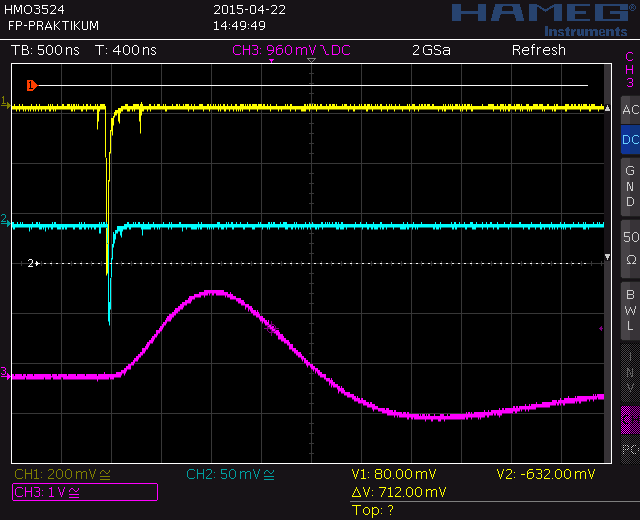
\includegraphics[width=0.5\textwidth]{../img/S0015.PNG}
  \caption{Signal from the linear gate (yellow), attenuated signal (blue) and signal after the shaping 
 amplifier (pink). The amplitude of this signal contains information about the energy of the muon.}
  \label{img:gateattshamp}
\end{center}
\end{figure}

To generate the control signal for the linear gate, additional units are necessary:
Two more scintillators with photomultipliers over and under the tank (PMt and PMb)
detect the approach (and the flight through) of muons.
Here again two discriminators are used to block small signals.
The discriminator levels are set to values which lead to about 200 counts per second.
After the discriminators, the signal is delayed by 25\,ns to keep in time with the other components
of the setup.

\autoref{img:tdiscdel} shows a pulse of 
the photomultiplier over the tank (yellow), the signal after the discriminator (blue) and
the delayed signal.

\begin{figure}[H]
\begin{center}
  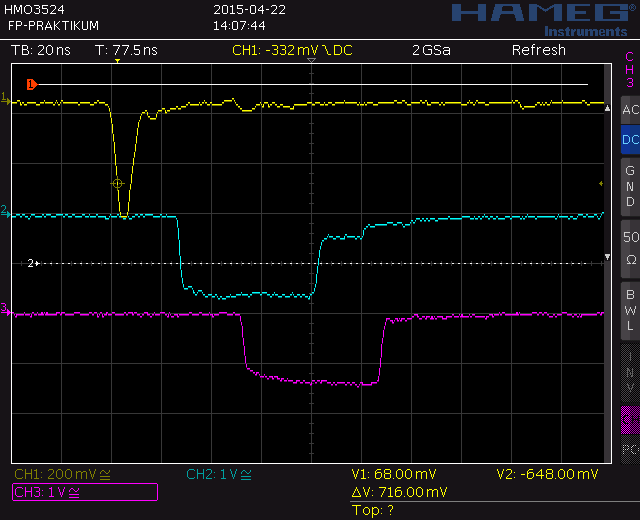
\includegraphics[width=0.5\textwidth]{../img/S0006.PNG}
  \caption{Signal from the photomultiplier over the tank (yellow), digital signal after the discriminator (blue)
  and delayed signal (pink).}
  \label{img:tdiscdel}
\end{center}
\end{figure}

The signal from the photomultiplier under the tank is processed the same way and
the signals from the two delay generators go into another coincidence unit (AND~II),
together with the output of AND~I. The inputs of AND~II can be switched off and on,
thus it can be defined which input conditions are necessary to trigger an output signal of AND~II.
The assignment of the inputs A, B and C can be seen on \autoref{img:setup}.
The counter Z~II counts the events after AND~II.
\autoref{img:discdiscandII} shows input (yellow and blue) and output signal (pink) of AND~II.

\begin{figure}[H]
\begin{center}
  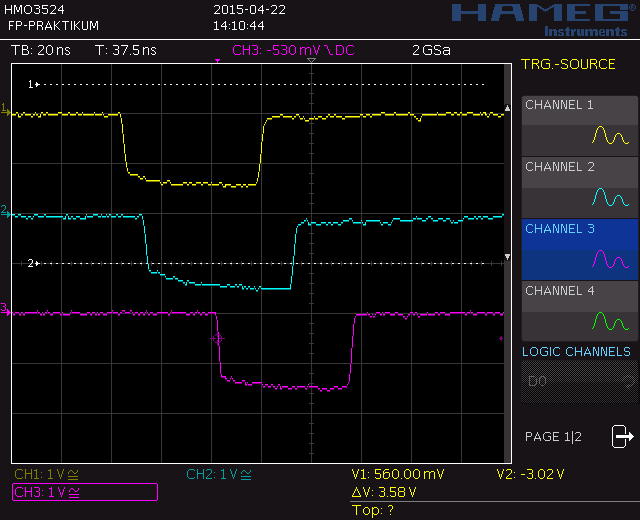
\includegraphics[width=0.5\textwidth]{../img/S0007.PNG}
  \caption{A muon flying through the tank causes two coinciding signals (yellow and blue) going
  into the coincidence unit AND II. The output signal is in pink.}
  \label{img:discdiscandII}
\end{center}
\end{figure}

The output signal of AND II is delayed by 500\,ns in a \emph{gate/delay generator}.
This delay is necessary to avoid the incorrect identification of a passing muon as a decaying muon
in a following section of the setup.
The gate/delay generator triggers the opening of a 7.5\,\textmu s wide window in the subsequent
\emph{timing unit}.
The signals are shown on \autoref{img:andIIgatetu}: The pulse after AND II in yellow,
the delayed pulse from the gate/delay generator in blue and the window of the timing unit in pink.

\begin{figure}[H]
\begin{center}
  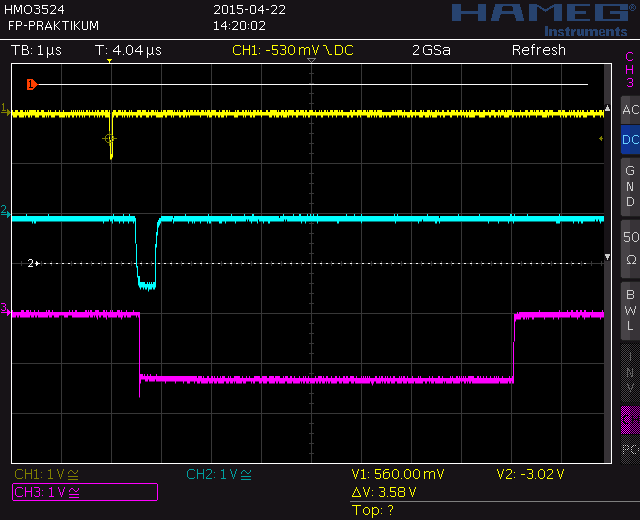
\includegraphics[width=0.5\textwidth]{../img/S0009.PNG}
  \caption{Pulse after the coincidence unit AND~II (yellow), delayed signal after the gate/delay generator (blue)
  and 7.5\,\textmu s-window of the timing unit (pink).}
  \label{img:andIIgatetu}
\end{center}
\end{figure}

The signal of the timing unit (which occurs once the intrusion of a muon in the tank is detected)
then goes into another coincidence unit AND~III (input A).
During the wide window of the timing unit the decay of the muon can cause a signal
of the coincidence unit AND~I. This signal also goes into AND~III
(yellow on \autoref{img:andItuIandIIItuII}).
After AND~III (pink),
another timing unit with a window of 400\,ns provides the opening signal for the linear gate (green).

For the flight through measurement it is possible to shortcut the gate/delay generator and the timing unit
and to pass the signal of AND~II directly into AND~III (input B).

Events of AND~III are counted with the counter Z~III.

\begin{figure}[H]
\begin{center}
  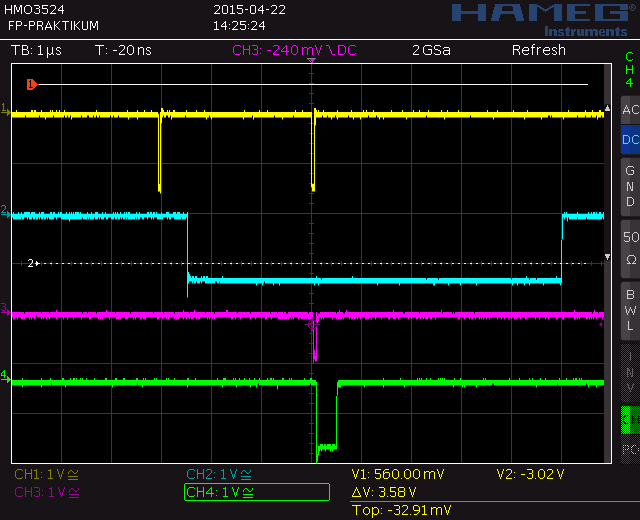
\includegraphics[width=0.5\textwidth]{../img/S0010.PNG}
  \caption{Creation of the control signal for the linear gate (green):
  The coincidence unit AND~I records two events (yellow), the first event arising from the intrusion
  of a muon in the tank. This triggers a wide window of the timing unit~I (blue) which
  allows the second pulse of AND~I due to the decay of the muon to pass through AND~III (pink).
  The signal of AND~III opens a window after the timing unit~II (green).}
  \label{img:andItuIandIIItuII}
\end{center}
\end{figure}

For the measurement of the decay time of muons a \emph{time to amplitude converter} is used.
It provides a signal whose amplitude is proportional to the time difference between a start and a stop signal.
The start signal is delivered by the coincidence unit AND~II when a muon enters the tank.
The stop signal comes from AND~III when a decay is recorded.
The output of the TAC goes into a multi channel analyzer which is connected to a computer.
The signals for and from the TAC are shown on \autoref{img:tac}.\\

To perform the time calibration of the TAC, a special device is provided to generate start and stop
pulses with adjustable time difference.\\

For the determination of the energy resolution of the setup a LED is integrated in the tank.
The LED is controlled with a pulse generator and a LED driver.


\begin{figure}[H]
\begin{center}
  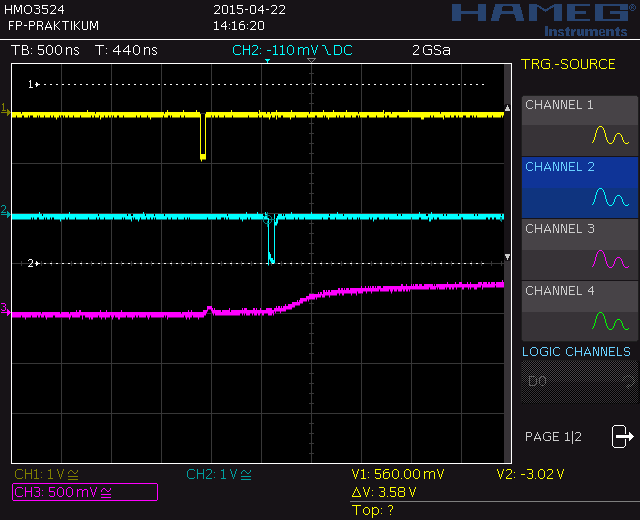
\includegraphics[width=0.5\textwidth]{../img/S0008.PNG}
  \caption{Signals at the time to amplitude converter: Start (yellow), stop (blue) and output (pink).}
  \label{img:tac}
\end{center}
\end{figure}

To verify the correct operation of the system after setting it up and during the days of the measurements,
the count rates of the four photomultipliers and the coincident events were monitored regularly.
\autoref{tab:countrates} shows the values that were determined after the successful completion of the setup.

\begin{table}[H]
\caption{Count rates at various configurations of the setup.}
\begin{center}
\begin{tabular}{|c||c|c|c|c|c|c|}
  \hline 
  					& counter	& AND I	& AND II	& AND III	& counts				& count rate\footnotemark/ s$^{-1}$			\\ \hline \hline
  PMr				& Z I		& A		& -			& -			& 141443/100\,s			& \textbf{1414\,$\pm$\,4}					\\ \hline
  PMl				& Z I		& B		& -			& -			& 78865/100\,s			& \textbf{789\,$\pm$\,3}					\\ \hline
  PMt				& Z II		& -		& A			& -			& 16640/100\,s			& \textbf{166.4\,$\pm$\,1.3}				\\ \hline
  PMb				& Z II		& -		& B			& -			& 17181/100\,s			& \textbf{171.8\,$\pm$\,1.3}				\\ \hline
  PMr \& PMl		& Z I		& A B	& -			& -			& 106649/1000\,s		& \textbf{106.7\,$\pm$\,0.3}				\\ \hline
  PMt \& PMb		& Z II		& -		& A B		& -			& 108/100\,s			& \textbf{1.08\,$\pm$\,0.10}				\\ \hline
  t \& r \& l		& Z III		& A B	& A	C		& B C		& 20990/1000\,s			& \textbf{20.99\,$\pm$\,0.14}				\\ \hline
  t \& b \& r \& l  & Z III		& A B	& A	B C		& B C		& 973/1000\,s			& \textbf{0.97\,$\pm$\,0.03}				\\ \hline
  decays			& Z III		& A B	& A	C		& A C		& 213/1000\,s			& \textbf{0.213\,$\pm$\,0.014}				\\ \hline
  underground\footnotemark		& Z III		& A B	& A	C		& A C		& 16/1000\,s			& \textbf{0.016\,$\pm$\,0.004}				\\ \hline
\end{tabular}
\end{center}
\label{tab:countrates}
\end{table}

\addtocounter{footnote}{-1}
\footnotetext{The errors were calculated with Gaussian uncertainty propagation,
assuming a Poisson distribution of the error on the number of counts (see section \ref{subsub:errorcountrate}).}
\addtocounter{footnote}{1}
\footnotetext{For the measurement of the underground, the gate/delay time was increased by a factor of 100.}	

photomult description from szint-prot? oder in principles?
